In order to create a basis for the engine choice, similar aircraft were examined and the engine choices that went into them. Aircraft such as the Boeing 777-300, \textbf{crap crap}, and \textbf{crap crap}.

The following engines, seen below, are used in similar aircraft with great success: \hl{\textbf{engine 1}, \textbf{engine 2}, and \textbf{engine 3}.} \textit{Proceed to describe the engines and the pros and cons of each}

After initial sizing has been generated by the team, it will then be possible to use the generated values in order to form a power requirement guideline for the propulsion system. This power requirement will be the primary driver for the choice of an engine as it will ensure that the engine chosen is not overpowered and that it will perform as necessary as well.  

Talk about decision to go with two turbofan engine. Talk about philosophy basing engine off of 737 MAX and 777 X and other similar aircraft. We want a high bypass engine. Composite blades.

\begin{figure} [h!]
    \centering
    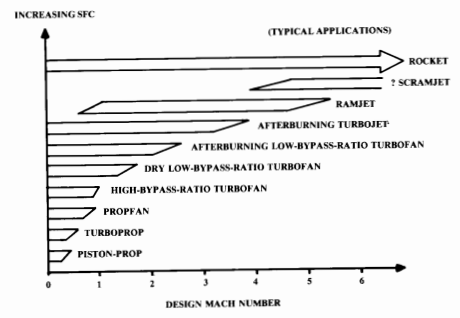
\includegraphics[width=0.8\textwidth]{Photos/PropSelection.PNG}
    \caption{Crap Crap from Raymer}
    \label{PropSelection}
\end{figure}

%% Or...:
% \begin{wrapfigure}{r}{0.5\textwidth}
%     \centering
%     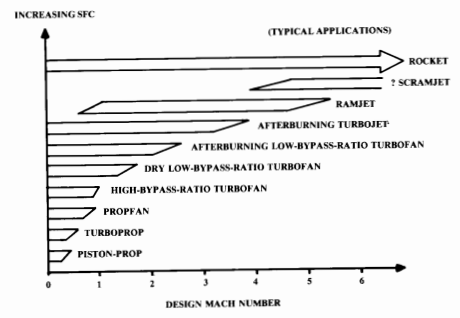
\includegraphics[width=0.5\textwidth]{Photos/PropSelection.PNG}
%     \caption{Caption}
%     \label{fig:my_label}
% \end{wrapfigure}

\textcolor{red}{
\begin{itemize}
    \item Discuss overall propulsion system philosophy/design/selection.
    \item Discuss future work.
    \item AIAA: Propulsion system description and characterization including performance,
    dimensions, and weights. The selection of the propulsion system(s), sizing, and
    airframe integration must be supported by analysis, trade studies, and discussion
\end{itemize}}